\documentclass[12pt]{beamer}
\usepackage{xeCJK}
\setCJKmainfont{蘋方-繁}
\renewcommand{\baselinestretch}{1.5}
\usepackage[T1]{fontenc}
\usetheme{CambridgeUS}
\usepackage[osf]{MinionPro}
\usepackage{MyriadPro}
\usecolortheme{beaver}

\newcommand*{\dif}{\,\mathrm{d}}
\newtheorem*{definition*}{Definition}
\newtheorem*{corollary*}{Corollary}
\def\tb#1#2{\mathop{#1\vphantom{\sum}}\limits_{\displaystyle #2}}
\usefonttheme{professionalfonts}

\usepackage{amsmath, amssymb, amsthm}
\newtheorem{prop}{\scshape Proposition}
\newenvironment{propc}[1]
{\begin{prop}}
        {\end{prop}}
\setbeamertemplate{theorems}[numbered]

\AtBeginSection[]{
  \begin{frame}
  \vfill
  \centering
  \begin{beamercolorbox}[sep=8pt,center,shadow=true,rounded=true]{title}
    \usebeamerfont{title}\insertsectionhead\par%
  \end{beamercolorbox}
  \vfill
  \end{frame}
}

\usepackage{tikz}
\usepackage{booktabs,tabulary}
\usepackage{threeparttable}

\title{Winning Rate of HearthStone Decks}
\author{陳柏瑜, 高翊傑}
\institute[NTU Econ]{\scshape ccClub2020 Fall\\ NTU Econ}
\date{2020.12.23}

\begin{document}
\begin{frame}
\titlepage
\end{frame}

\begin{frame}
\frametitle{Outline}
\tableofcontents
\end{frame}


\section{Background} 

%%%
\begin{frame}[fragile]{Hearthstone}

	\begin{figure}
		\begin{center}
			
\includegraphics[width=1\textwidth]{figure/f01.jpg}
		\end{center}
	\end{figure}

\end{frame}



%%%
\begin{frame}[fragile]{Hearthstone}

	\begin{figure}
		\begin{center}
			
\includegraphics[width=0.6\textwidth]{figure/f02-1.png}
		\end{center}
	\end{figure}

\end{frame}


%%%
\begin{frame}[fragile]{Hearthstone}

	\begin{figure}
		\begin{center}
			
\includegraphics[width=0.3\textwidth]{figure/f02-2.png}
		\end{center}
	\end{figure}

\end{frame}

%%%
\begin{frame}[fragile]{Hearthstone}

	\begin{itemize}
		\item 職業:
		\begin{enumerate}
			\item 惡魔獵人、德魯伊、獵人、法師、聖騎士、牧師、盜賊、薩滿、術士、戰士

		\end{enumerate}}

		\item 牌組:上千副乃至於更多(每三十張牌(cards)組成一副牌組(Deck))
		\item 常見類型:快攻、節奏、生物鋪場、死聲、Buff、一波帶走 \dots 等

	\end{itemize}
	
\end{frame}


\section{Core Question}

%%%
\begin{frame}[fragile]{Winning Rate of a deck}

	\begin{itemize}
		\item 給定任意一副牌組(i.e. 30張卡牌),這副牌牌組的勝率是多少?
	\end{itemize}
	
	考量其他影響勝率的因素:
	\begin{itemize}
		\item 職業
		\item 牌組造價(魔塵)
		\item 牌組節奏(一局遊戲的時長)
		\item 牌組遊玩局數(熱門程度)
	\end{itemize}

\end{frame}

\section{Data}

%%%
\begin{frame}[fragile]{HSReplay.net}
	
	在總共十個職業中,根據每個職業、在每週不定期紀錄以下資訊:
	\begin{itemize}
		\item 紀錄至少36副牌組的勝率
		\item 紀錄每副牌組的組成(其中30張卡分別是哪些卡)
		\item 每副牌組的造價(魔塵花費)
		\item 每副牌組節奏(一局遊戲的時長)
		\item 每副牌組的遊玩局數(至少對局200場以上)
	\end{itemize}

	其中,我們自2020-12-06起至2020-12-24每天爬取該網站,取得每副牌組的勝率紀錄

\end{frame}

%%%
\begin{frame}[fragile]{Scraped Data}

以 dictionary of dictionary 儲存牌組資訊

	\begin{figure}
		\begin{center}
			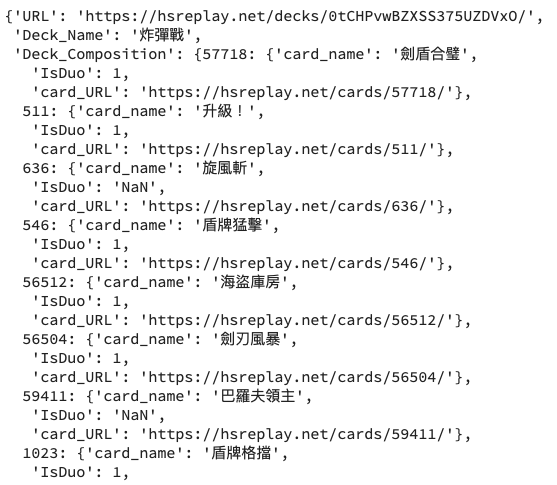
\includegraphics[width=0.5\textwidth]{figure/f03.png}
		\end{center}
	\end{figure}

\end{frame}


%%%
\begin{frame}[fragile]{Distinct Cards}

在標準環境中對戰的所有牌組共有973張相異的卡牌,其中有226張中立卡牌

	\begin{figure}
		\begin{center}
			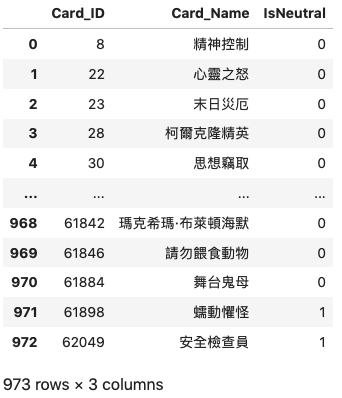
\includegraphics[width=0.3\textwidth]{figure/f04.png}
		\end{center}
	\end{figure}

\end{frame}


%%%
\begin{frame}[fragile]{Tidy Deck Data}

	\begin{figure}
		\begin{center}
			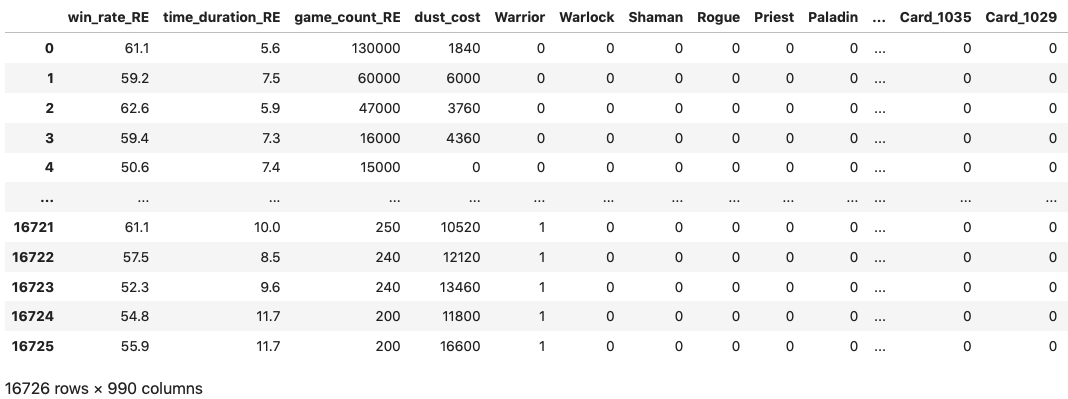
\includegraphics[width=1\textwidth]{figure/f05.png}
		\end{center}
	\end{figure}

\end{frame}

%%%
\begin{frame}[fragile]{Tidy Deck Data}

	\begin{itemize}
		\item 共有$16726$筆觀察值(不盡相同勝率的deck),990個feature
		\item dummy variables中有973個為個別卡牌、10個為職業
		\item variable of interest 為 win rate
		\item time duration, dust cost 皆為 continuous variable
		\item game count 為 discrete count data
		\item Deck URL、Deck ID分別為deck對應的網址以及ID
		\item Deck Name為牌組名稱(不唯一,不同組成的牌組可能有相同名稱)
	\end{itemize}


\end{frame}



\section{Model}

%%%
\begin{frame}[fragile]{Random Forest}

	相較於傳統的迴歸模型,決策樹模型可以給我們在「是否選擇把某張卡放進牌組裡」一個更好的詮釋

	我們將提供以下模型的估計:

	\begin{itemize}
		\item OLS result
		\item Random Forest
		\item Random Forest with PCA dimension reduction
	\end{itemize}

\end{frame}


\section{Result}

%%%
\begin{frame}[fragile]{Random Forest}

	相較於傳統的迴歸模型,決策樹模型可以給我們在「是否選擇把某張卡放進牌組裡」一個更好的詮釋

	我們將提供以下模型的估計:

	\begin{itemize}
		\item OLS
		\item LASSO
		\item Random Forest
		\item Random Forest with PCA dimension reduction
	\end{itemize}

\end{frame}


%%%
\begin{frame}[fragile]{Before Random Forest: OLS}

An OLS Model without specific cards: sketch the big picture of the meta

對於勝率有正相關的大致指標包含:

	\begin{itemize}
		\item 節奏快的牌組(天下武功,唯快不破?!)
		\item 造價高的牌組(有傳說、史詩)
		\item 熱門的牌組(比較多人愛抄)
		\item 天梯上比較常見的職業:惡魔獵人、獵人、聖騎士
	\end{itemize}
	有較高的勝率


\end{frame}

%%%
\begin{frame}[fragile]{Before Random Forest: OLS}

	\begin{figure}
		\begin{center}
			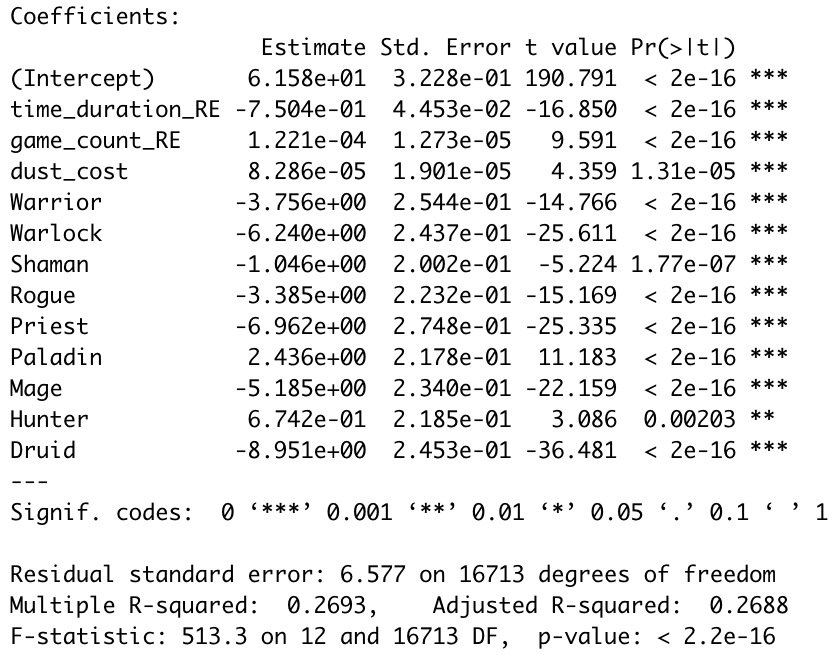
\includegraphics[width=0.7\textwidth]{figure/f06.png}
		\end{center}
	\end{figure}

\end{frame}

%%%
\begin{frame}[fragile]{Before Random Forest: OLS after control}

	\begin{figure}
		\begin{center}
			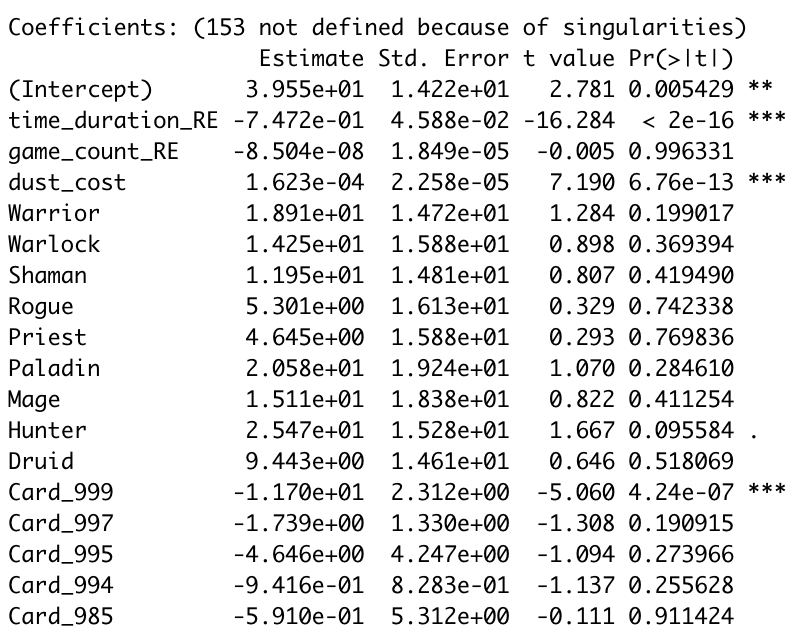
\includegraphics[width=0.6\textwidth]{figure/f07.png}
		\end{center}
	\end{figure}


\end{frame}

%%%
\begin{frame}[fragile]{Before Random Forest: OLS after control}

在以放入哪些卡牌作為控制變數後,可以看見仍是

	\begin{itemize}
		\item 節奏快的牌組(天下武功,唯快不破?!)
		\item 造價高的牌組(有傳說、史詩)
	\end{itemize}
	有較高的勝率

當然,此時我們便面對了 the curse of high dimensionality

\end{frame}



%%%
\begin{frame}[fragile]{Before Random Forest: LASSO}

一個自然的解決方式是用penalty regression;透過cross validation選擇tuning parameter $\lambda$後,便可得到:

%  [1] win_rate          4.67218665473637    
%  [2] time_duration     0.000156656548294709
%  [3] Card_62049        0.832009763102095
%  [4] Card_60280        2.55282958928911
%  [5] Card_59658        0.15411656900678
%  [6] Card_59646        -1.49511713454943
%  [7] Card_59395        4.34942441528714
%  [8] Card_59039        1.76100661192004
%  [9] Card_59036        1.78894309462431
% [10] Card_59035        1.48871453526339
% [11] Card_58973        2.26300441482049
% [12] Card_55429        2.16930380979627
% [13] Card_55401        1.09320992464284
% [14] Card_53771        1.78211572392716
% [15] Card_48           0.78900693038165

	\begin{figure}
		\begin{center}
			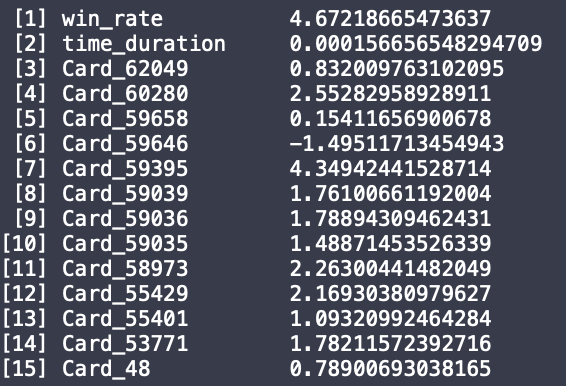
\includegraphics[width=0.6\textwidth]{figure/f09.png}
		\end{center}
	\end{figure}

\end{frame}


%%%
\begin{frame}[fragile]{Before Random Forest: LASSO}

翻譯過來就是:

%  [1] win_rate          4.67218665473637    
%  [2] time_duration     0.000156656548294709
%  [3] 安全檢查員          0.832009763102095
%  [4] 盤牙督軍            2.55282958928911
%  [5] 維克圖斯            0.15411656900678
%  [6] 魔杖師             -1.49511713454943
%  [7] 模範生史黛琳娜       4.34942441528714
%  [8] 愛玩筆的學生        1.76100661192004
%  [9] 討人厭的教師        1.78894309462431
% [10] 導覽員             1.48871453526339
% [11] 火爆的赤紅龍人      2.26300441482049
% [12] 閃避飛龍           2.16930380979627
% [13] 盜匪傘兵           1.09320992464284
% [14] 托爾托朝聖者        1.78211572392716
% [15] 虛無行者           0.78900693038165
	\begin{figure}
		\begin{center}
			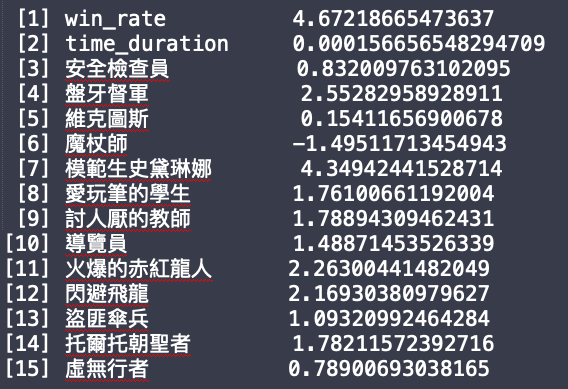
\includegraphics[width=0.6\textwidth]{figure/f10.png}
		\end{center}
	\end{figure}

\end{frame}


%%%
\begin{frame}[fragile]{Random Forest}

透過Random Forest,我們得到:
	\begin{figure}
		\begin{center}
			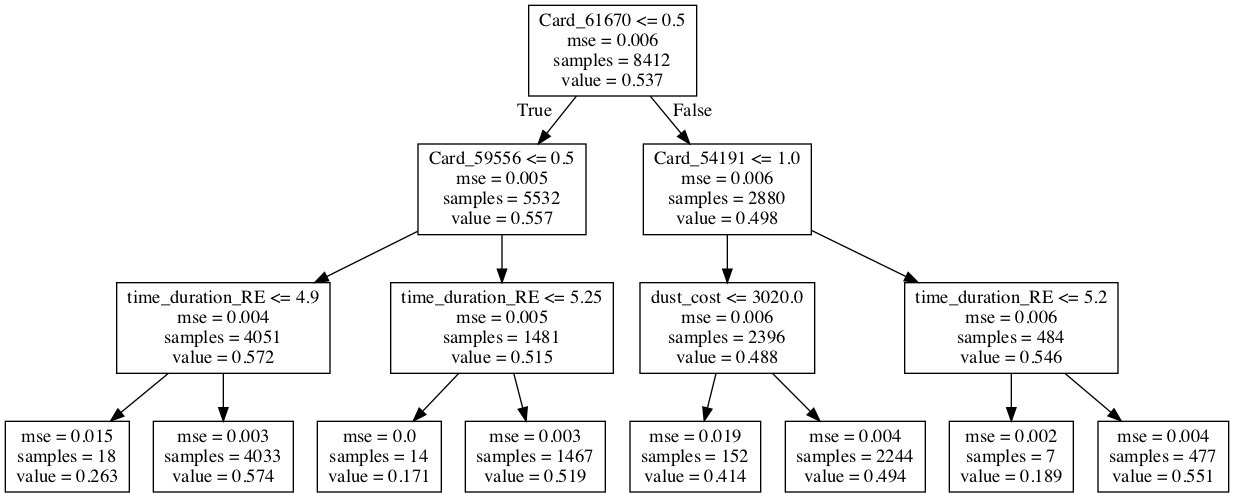
\includegraphics[width=0.9\textwidth]{figure/plot/1a.png}
		\end{center}
	\end{figure}

\end{frame}

%%%
\begin{frame}[fragile]{Random Forest}

	\begin{figure}
		\begin{center}
			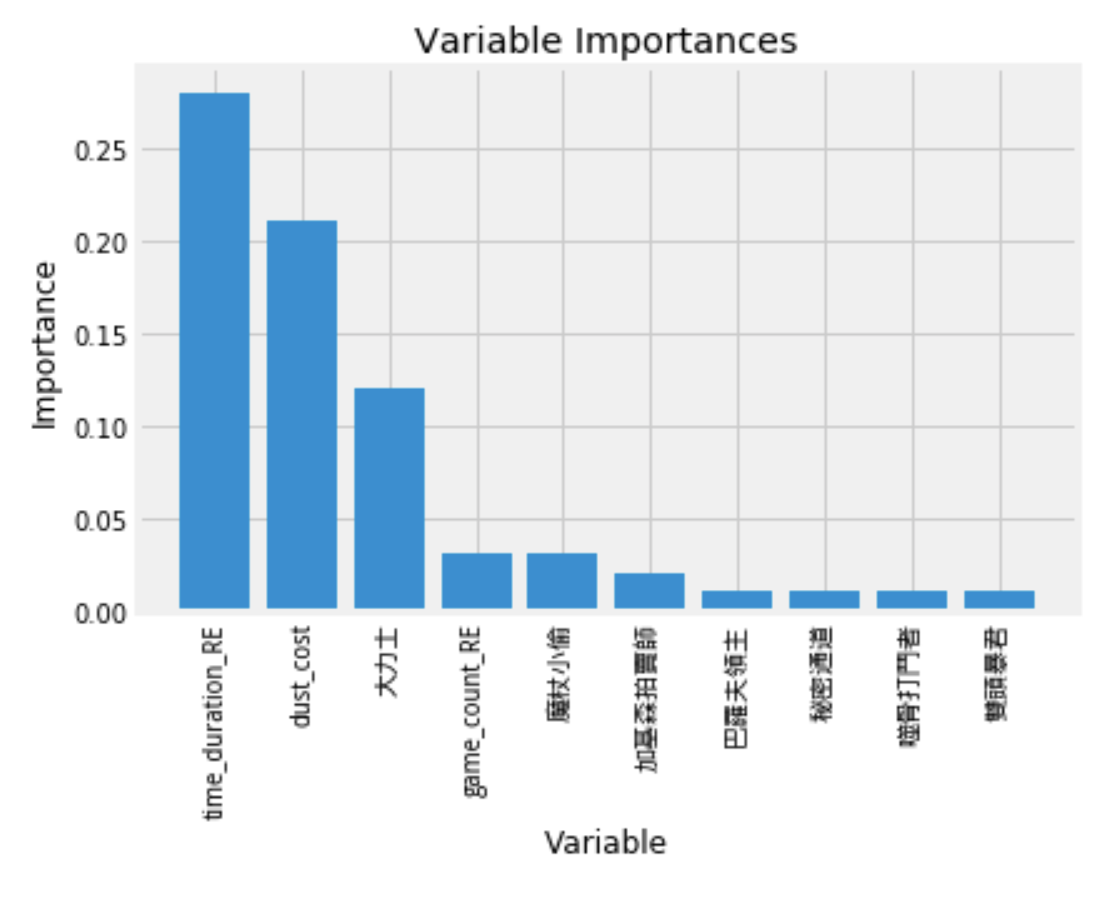
\includegraphics[width=0.8\textwidth]{figure/plot/1a_importance.png}
		\end{center}
	\end{figure}

\end{frame}

%%%
\begin{frame}[fragile]{Random Forest}

然而我們仍然擔心會有 the curse of high dimensionality 的問題,因此針對所有的卡牌(共973張)做PCA,即:

夠過PCA將973張卡牌做dimension reduction,期望能得到extracted information


\end{frame}


%%%
\begin{frame}[fragile]{Random Forest with PCA}

	\begin{figure}
		\begin{center}
			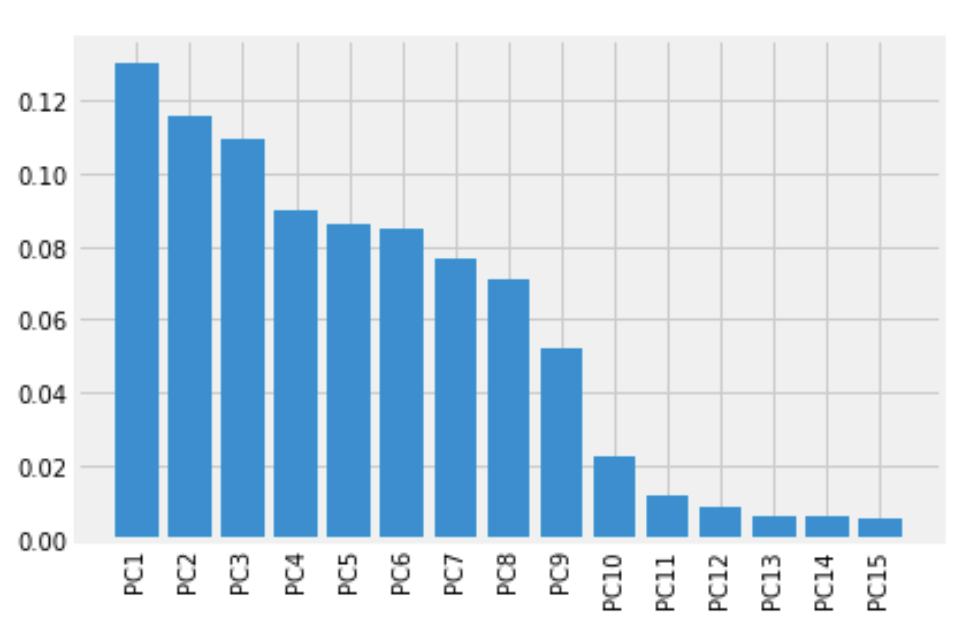
\includegraphics[width=0.8\textwidth]{figure/plot/2b.png}
		\end{center}
	\end{figure}

\end{frame}

%%%
\begin{frame}[fragile]{Random Forest with PCA}

	\begin{figure}
		\begin{center}
			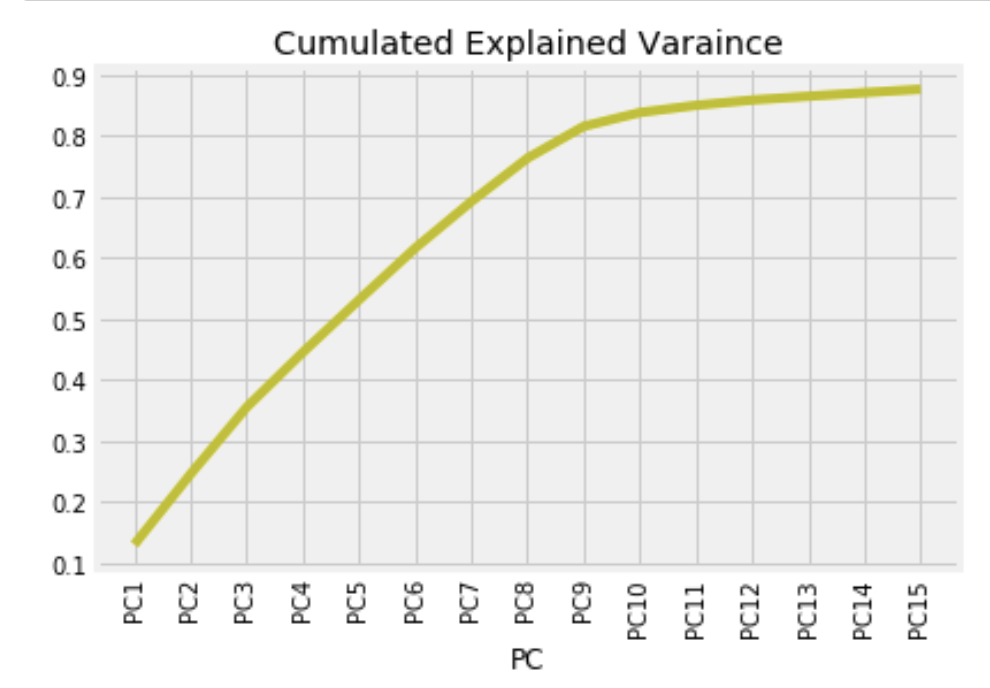
\includegraphics[width=0.8\textwidth]{figure/plot/2c.png}
		\end{center}
	\end{figure}

\end{frame}


%%%
\begin{frame}[fragile]{Random Forest with PCA}

	\begin{figure}
		\begin{center}
			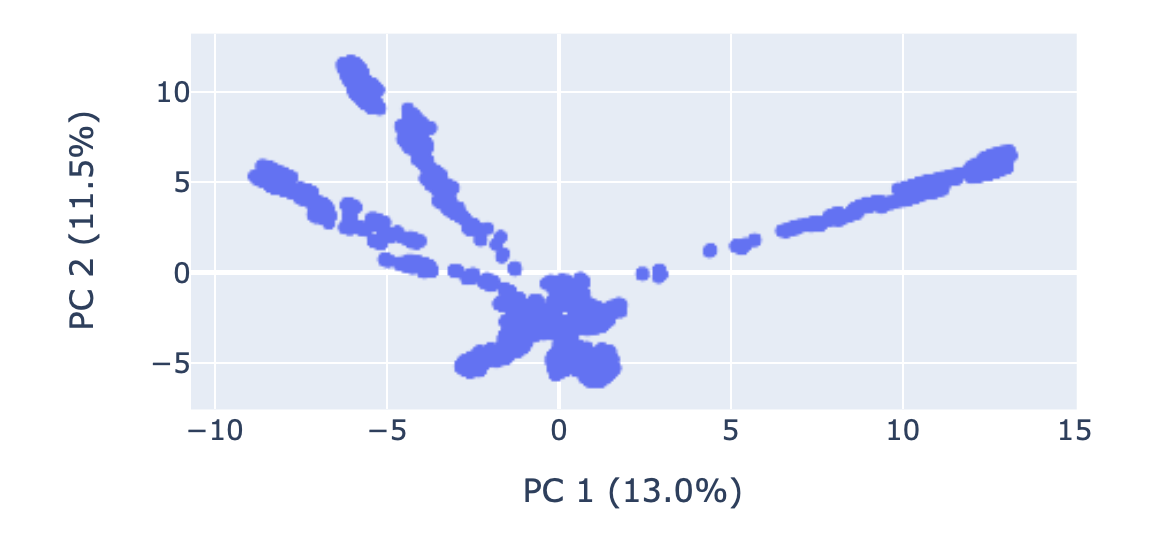
\includegraphics[width=0.8\textwidth]{figure/plot/2d.png}
		\end{center}
	\end{figure}

	放射狀?

\end{frame}

%%%
\begin{frame}[fragile]{Random Forest with PCA: 職業 dependent 惡魔獵人}
	\begin{figure}
		\begin{center}
			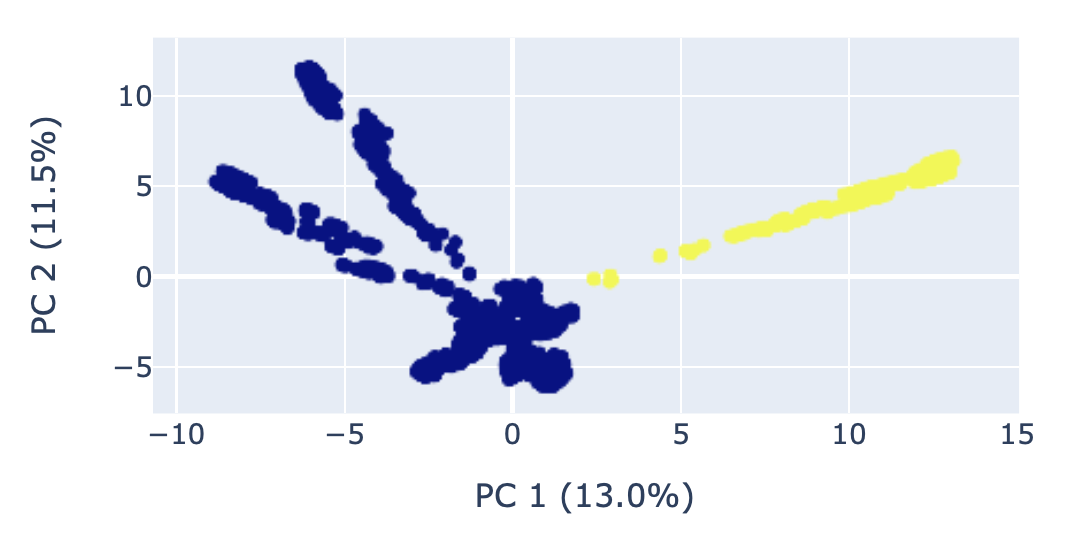
\includegraphics[width=0.8\textwidth]{figure/plot/2_DH.png}
		\end{center}
	\end{figure}
\end{frame}
%%%
\begin{frame}[fragile]{Random Forest with PCA: 職業 dependent 德魯伊}
	\begin{figure}
		\begin{center}
			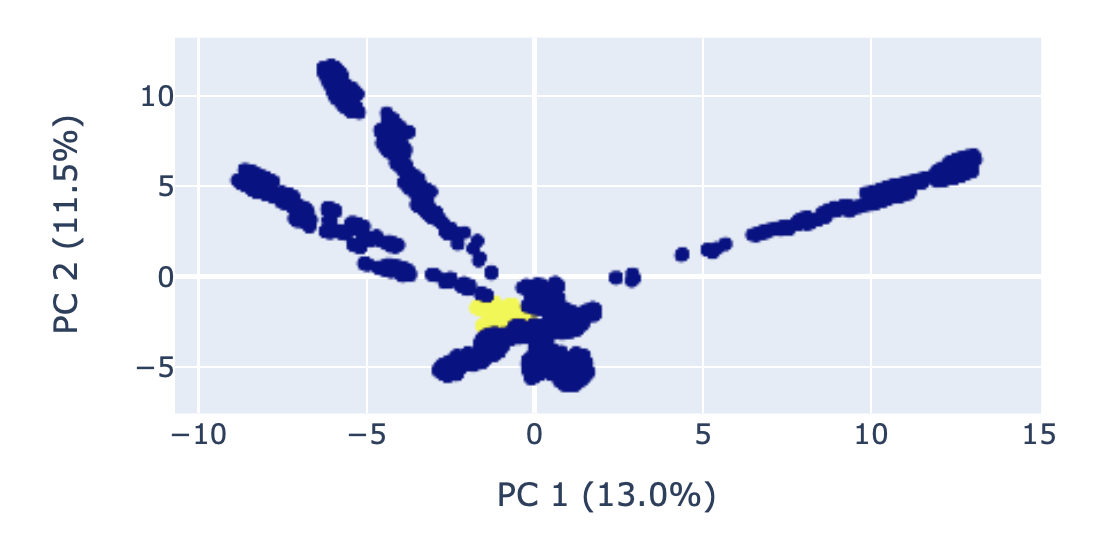
\includegraphics[width=0.8\textwidth]{figure/plot/2_Druid.png}
		\end{center}
	\end{figure}
\end{frame}
%%%
\begin{frame}[fragile]{Random Forest with PCA: 職業 dependent 獵人}
	\begin{figure}
		\begin{center}
			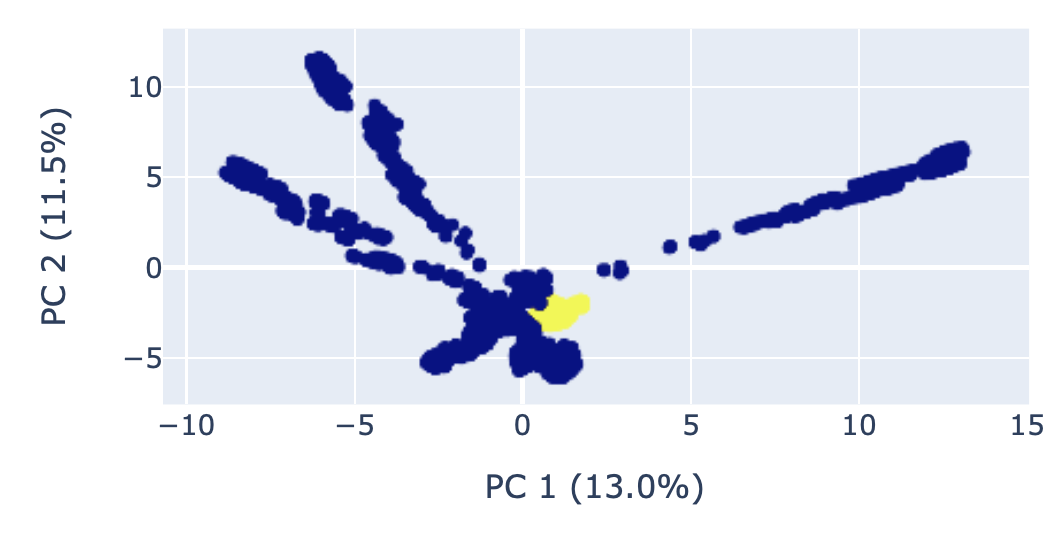
\includegraphics[width=0.8\textwidth]{figure/plot/2_hunter.png}
		\end{center}
	\end{figure}
\end{frame}
%%%
\begin{frame}[fragile]{Random Forest with PCA: 職業 dependent 法師}
	\begin{figure}
		\begin{center}
			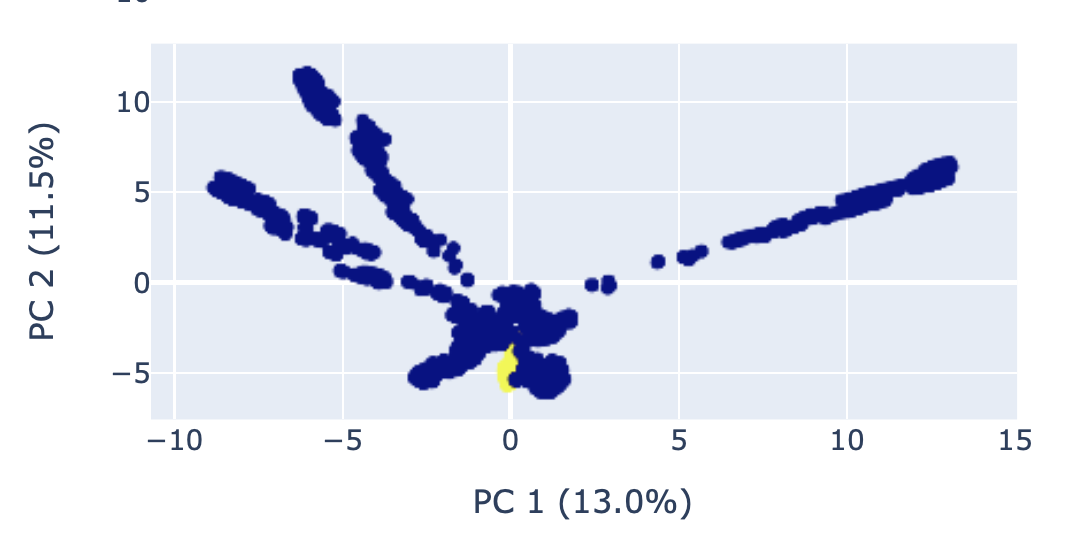
\includegraphics[width=0.8\textwidth]{figure/plot/2_mage.png}
		\end{center}
	\end{figure}
\end{frame}
%%%
\begin{frame}[fragile]{Random Forest with PCA: 職業 dependent 聖騎士}
	\begin{figure}
		\begin{center}
			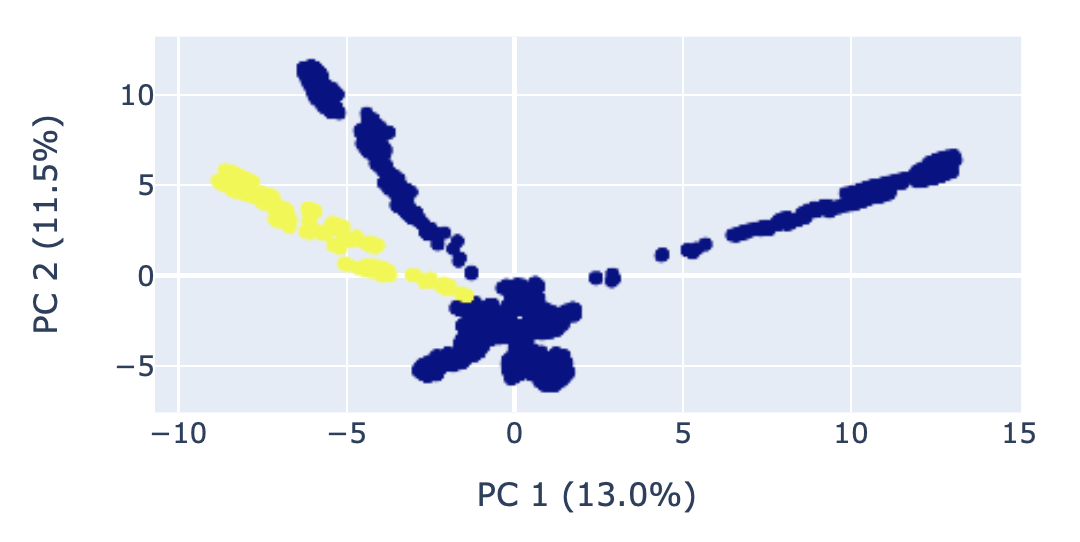
\includegraphics[width=0.8\textwidth]{figure/plot/2_paladin.png}
		\end{center}
	\end{figure}
\end{frame}
%%%
\begin{frame}[fragile]{Random Forest with PCA: 職業 dependent 盜賊}
	\begin{figure}
		\begin{center}
			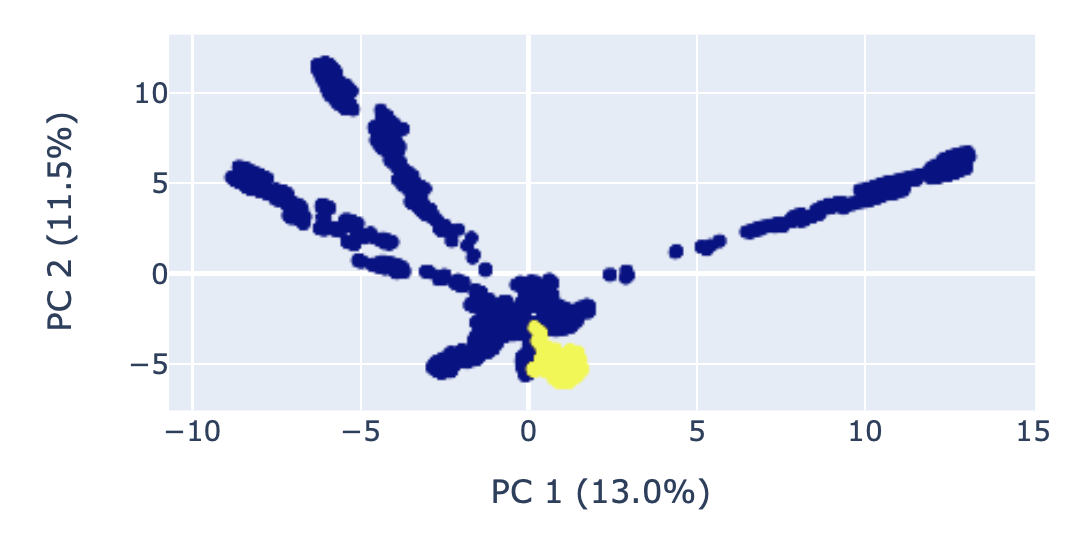
\includegraphics[width=0.8\textwidth]{figure/plot/2_rouge.png}
		\end{center}
	\end{figure}
\end{frame}
%%%
\begin{frame}[fragile]{Random Forest with PCA: 職業 dependent 薩滿}
	\begin{figure}
		\begin{center}
			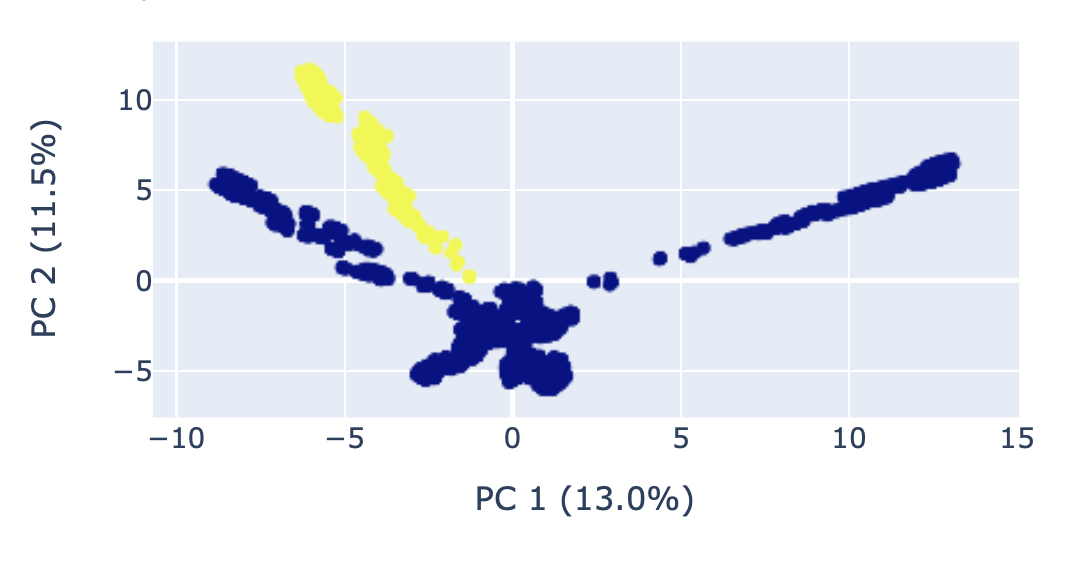
\includegraphics[width=0.8\textwidth]{figure/plot/2_shaman.png}
		\end{center}
	\end{figure}
\end{frame}
%%%
\begin{frame}[fragile]{Random Forest with PCA: 職業 dependent 術士}
	\begin{figure}
		\begin{center}
			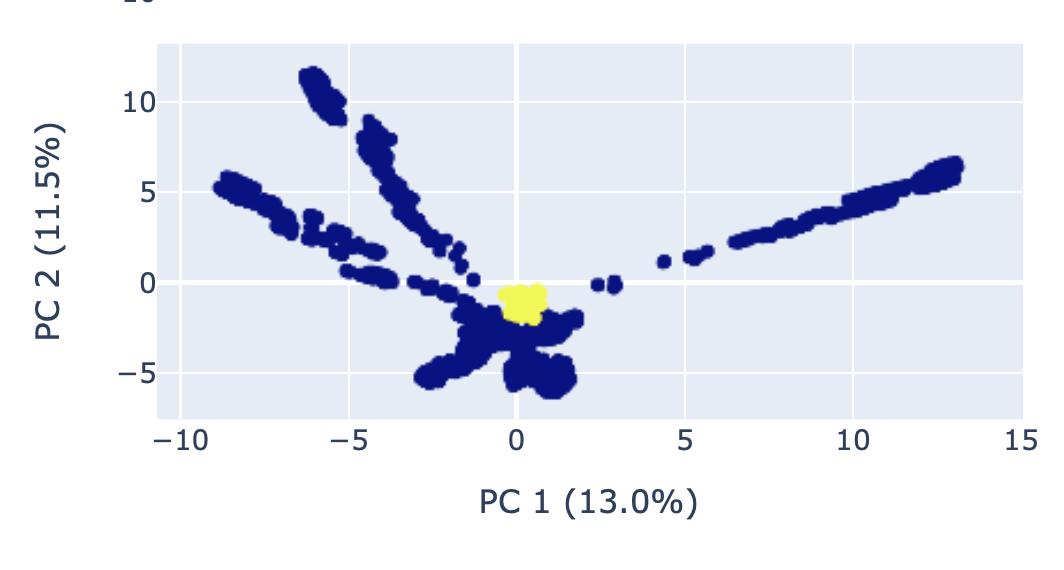
\includegraphics[width=0.8\textwidth]{figure/plot/2_warlock.png}
		\end{center}
	\end{figure}
\end{frame}
%%%
\begin{frame}[fragile]{Random Forest with PCA: 職業 dependent 戰士}
	\begin{figure}
		\begin{center}
			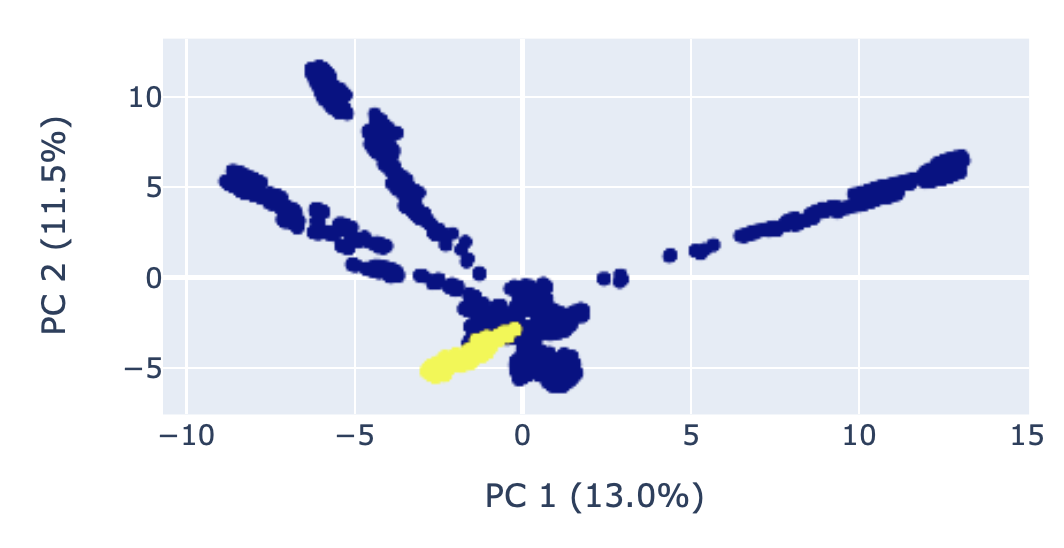
\includegraphics[width=0.8\textwidth]{figure/plot/2_warriro.png}
		\end{center}
	\end{figure}
\end{frame}


%%%
\begin{frame}[fragile]{Random Forest with PCA}

Hard to explain...

	\begin{figure}
		\begin{center}
			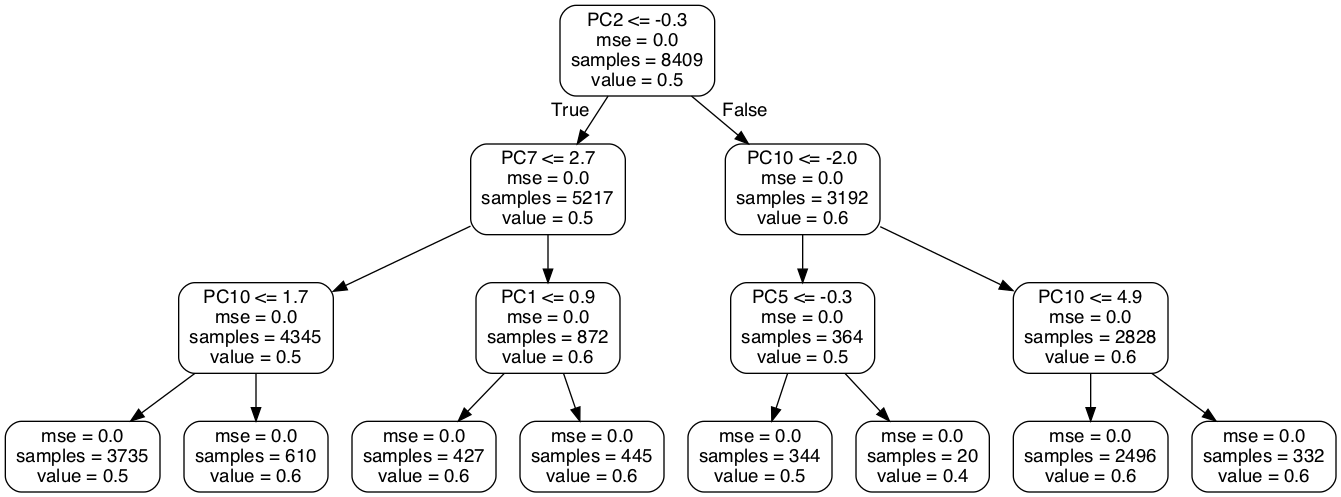
\includegraphics[width=0.9\textwidth]{figure/plot/2a.png}
		\end{center}
	\end{figure}

\end{frame}



%%%
\begin{frame}[fragile]{Random Forest with PCA: For Neutral Cards}

To avoid mixing up 職業 and 職業專屬卡牌

	\begin{figure}
		\begin{center}
			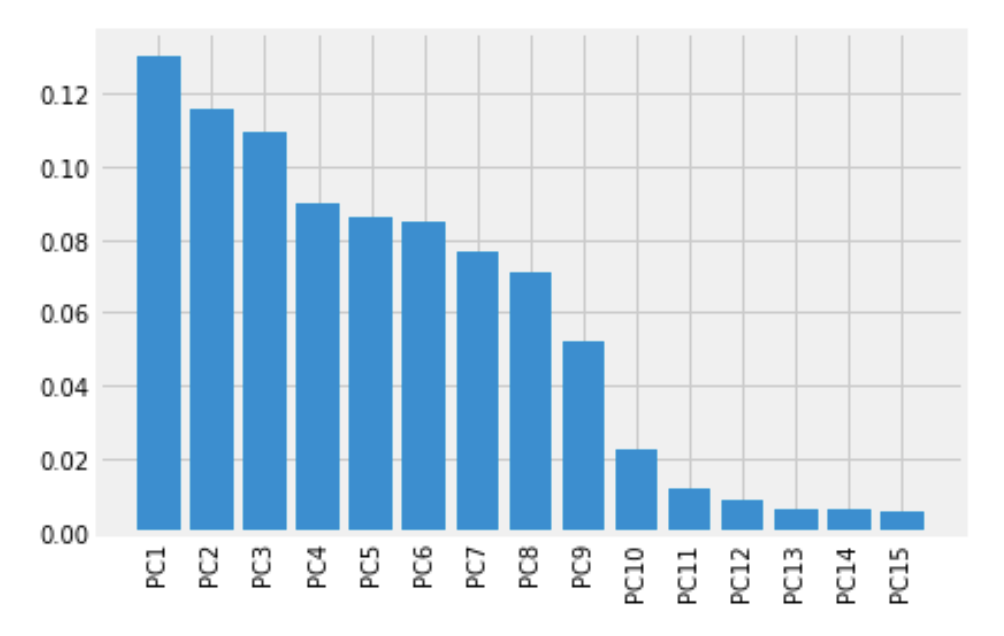
\includegraphics[width=0.8\textwidth]{figure/plot/3b.png}
		\end{center}
	\end{figure}

\end{frame}

%%%
\begin{frame}[fragile]{Random Forest with PCA: For Neutral Cards}

To avoid mixing up 職業 with 職業專屬卡牌

	\begin{figure}
		\begin{center}
			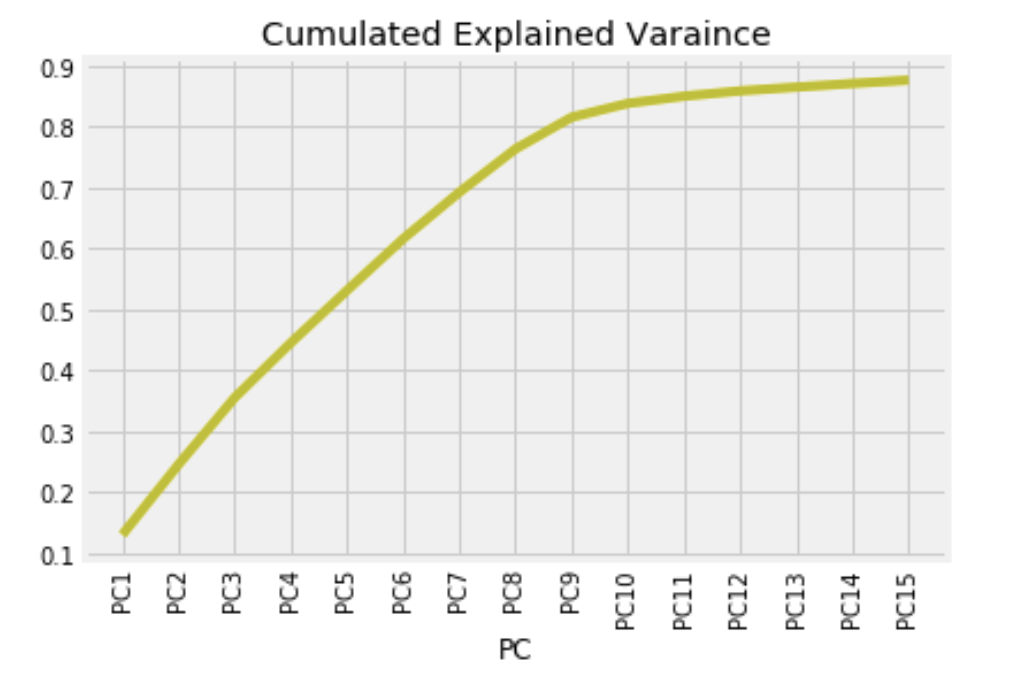
\includegraphics[width=0.8\textwidth]{figure/plot/3c.png}
		\end{center}
	\end{figure}

\end{frame}


%%%
\begin{frame}[fragile]{Random Forest with PCA: For Neutral Cards}

Plot the deck names

	\begin{figure}
		\begin{center}
			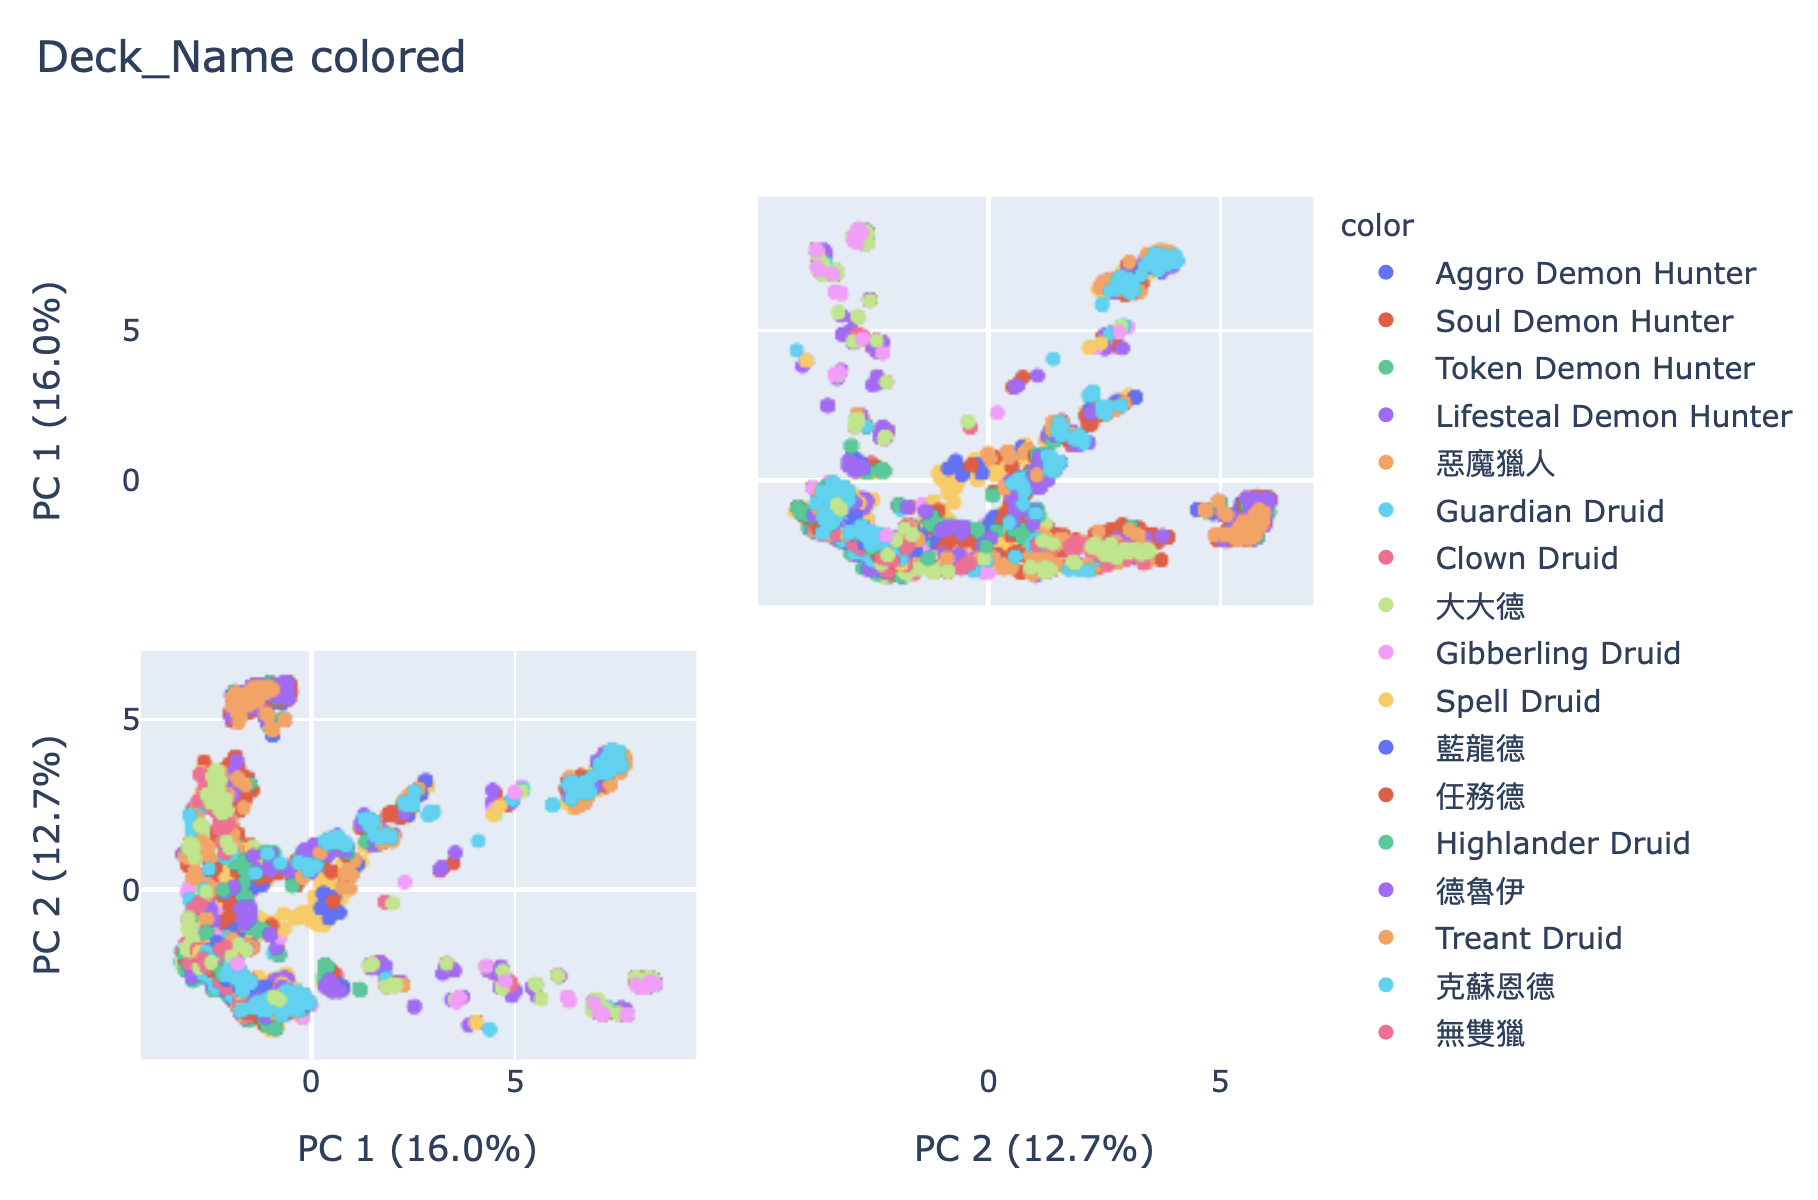
\includegraphics[width=0.8\textwidth]{figure/plot/3_deckname.png}
		\end{center}
	\end{figure}

\end{frame}

%%%
\begin{frame}[fragile]{Random Forest with PCA: For Neutral Cards}

Check the gif

\end{frame}

%%%
\begin{frame}[fragile]{Random Forest with PCA: For Neutral Cards}

labeling dust cost

	\begin{figure}
		\begin{center}
			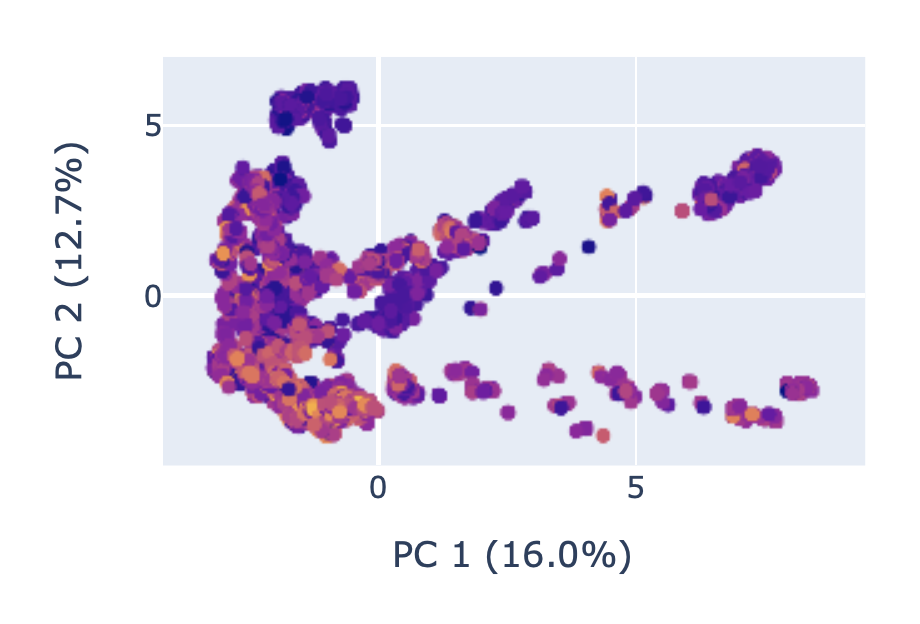
\includegraphics[width=0.8\textwidth]{figure/plot/3d_dust_cost.png}
		\end{center}
	\end{figure}

\end{frame}

%%%
\begin{frame}[fragile]{Random Forest with PCA: For Neutral Cards}

labeling time duration

	\begin{figure}
		\begin{center}
			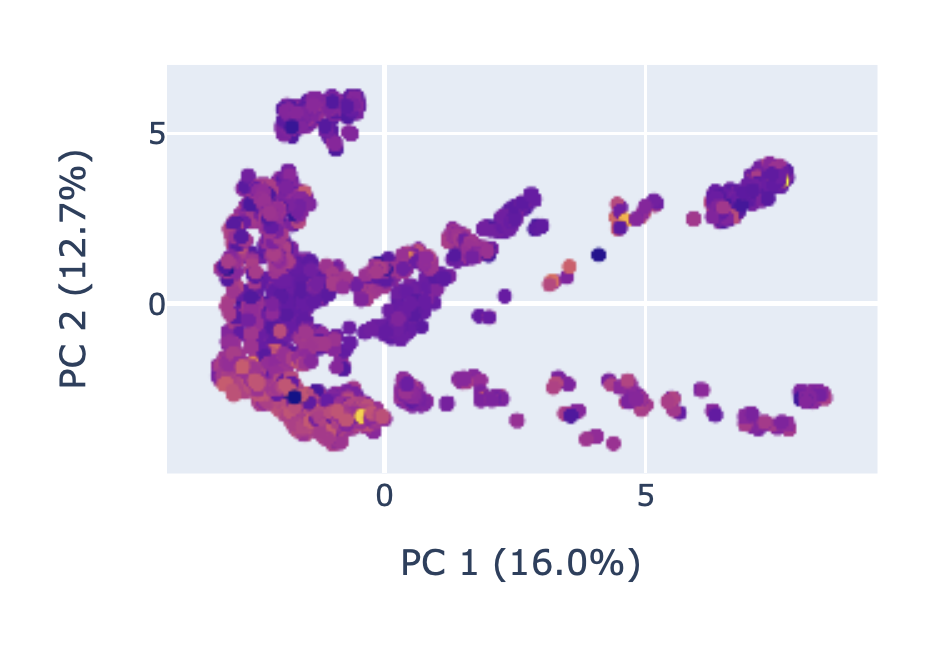
\includegraphics[width=0.8\textwidth]{figure/plot/3e_time_duration.png}
		\end{center}
	\end{figure}

\end{frame}

%%%
\begin{frame}[fragile]{Random Forest with PCA: For Neutral Cards}

	\begin{figure}
		\begin{center}
			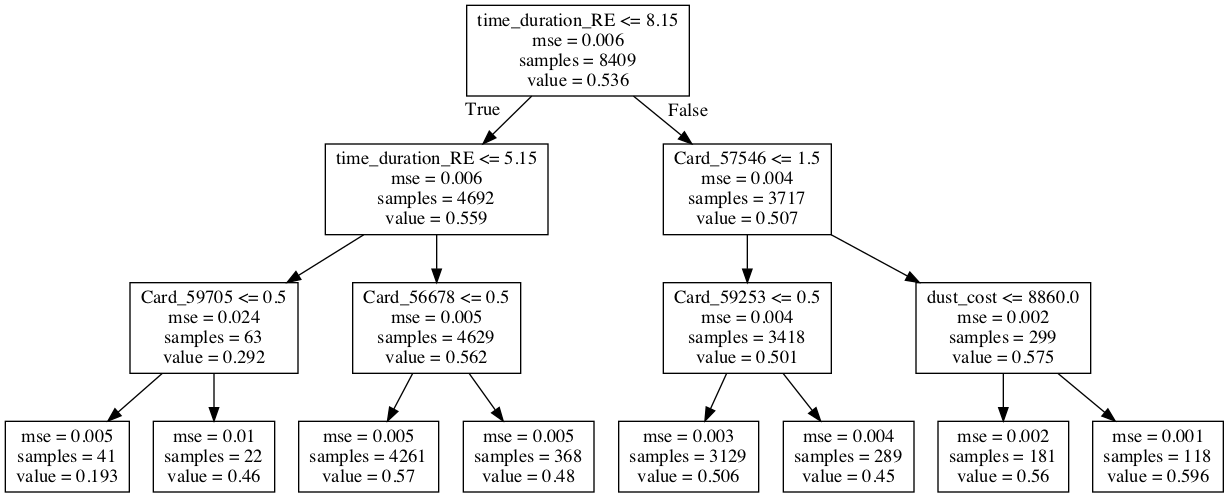
\includegraphics[width=0.9\textwidth]{figure/plot/3a.png}
		\end{center}
	\end{figure}

\end{frame}

%%%
\begin{frame}[fragile]{Random Forest with PCA: For Neutral Cards}

	\begin{figure}
		\begin{center}
			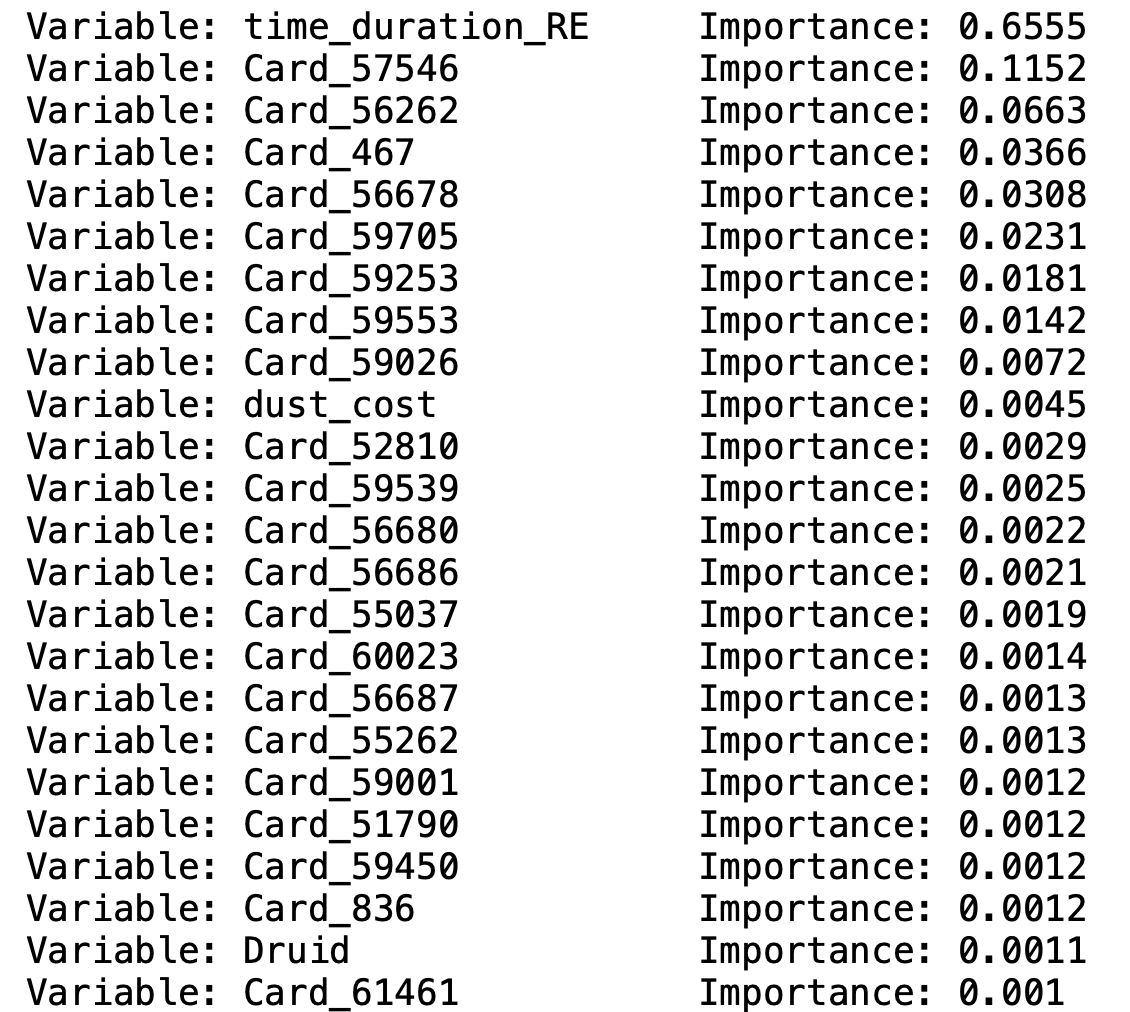
\includegraphics[width=0.6\textwidth]{figure/plot/3a_importance.png}
		\end{center}
	\end{figure}

\end{frame}


%%%
\begin{frame}[fragile]{Random Forest with PCA: For Neutral Cards}

	\begin{figure}
		\begin{center}
			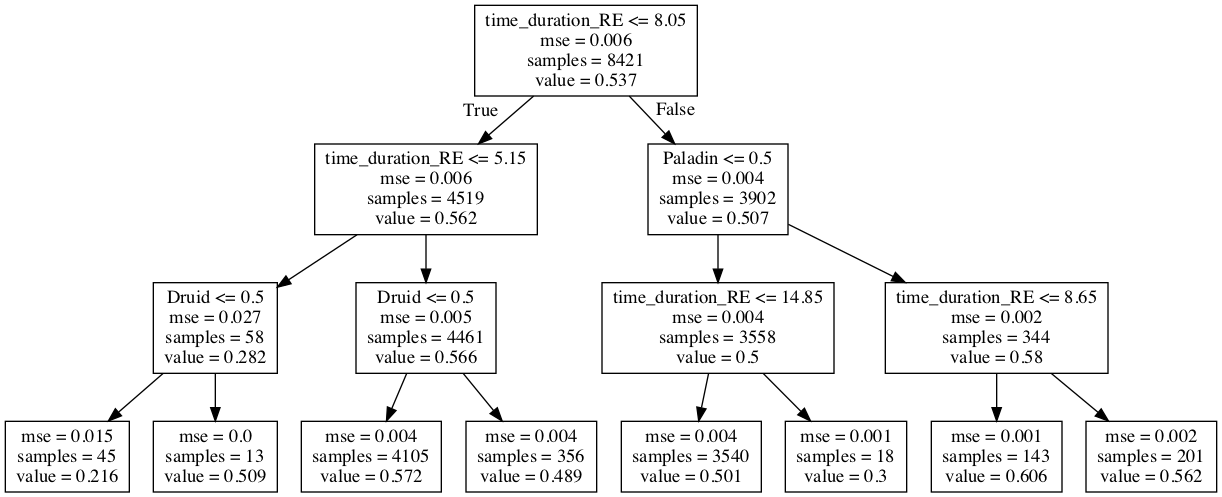
\includegraphics[width=0.9\textwidth]{figure/plot/3a_no_hero.png}
		\end{center}
	\end{figure}

\end{frame}

%%%
\begin{frame}[fragile]{Random Forest with PCA: For Neutral Cards}

	\begin{figure}
		\begin{center}
			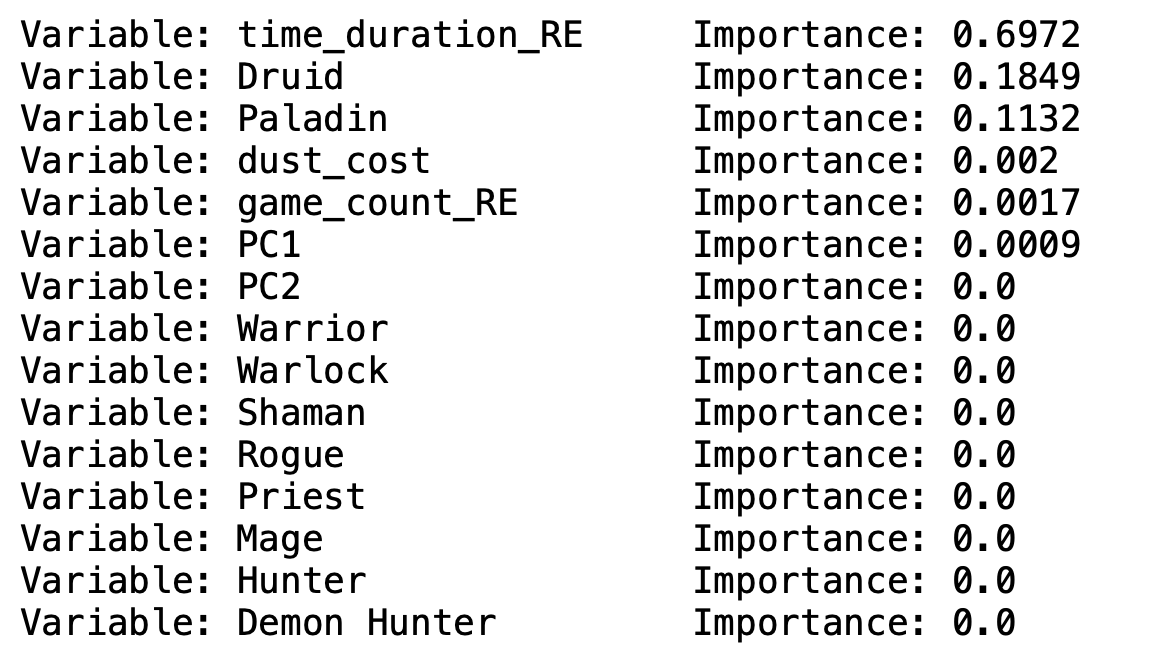
\includegraphics[width=0.7\textwidth]{figure/plot/3a_no_hero_importance.png}
		\end{center}
	\end{figure}

\end{frame}



\section{Conclusion}

%%%
\begin{frame}[fragile]{Conclusion}

	\begin{itemize}
		\item A baseline model (only using a fixed sample mean to predict the winning rate) predicts a fixed $53\%$ winning rate.
		\item Even a OLS model induce that same conclusion that time duration is most important feature.
		\item A certain card may play an important role in a deck, but the composition plays a more important role.
		\item The cost of a deck matters, but not a lot.
	\end{itemize}

\end{frame}


\section{Further Topic}

%%%
\begin{frame}[fragile]{Next Step...}

	經過以上分析,我們仍有以下幾處問題尚待解決:

	\begin{itemize}
		\item A better model selection decision for a tree-based model
		\item the validity of a continuous / discrete variable in Random Forest
		\item Random Forest with PCA dimension reduction
		\item There may exist a more reliable model for modeling the distribution of the winning rate
	\end{itemize}

\end{frame}




\end{document}